\documentclass[a4paper,12pt]{article}
\usepackage{enumerate,amsmath,graphicx,float,epstopdf,subcaption}
\graphicspath{ {./} }
\usepackage{verbatim}

\begin{document}

\title{PHY566 Group Project 2 \\ 
	Eco-system: Predator and Prey}
\date{\today}
\author{David Hicks\\ Weiyao Ke \\ Shagun Maheshwari \\ Fan Zhang}

\maketitle
\section{Abstract}

The following is the link to the GitHub account of the work done in this paper: \\
\begin{center}
https://github.com/keweiyao/Project-B-PHY566.git
\end{center}

\section{Introduction to eco-system modelling}
The dynamics of biological systems consist of one predator and one prey can be described by Lotka-Volterra equations:
\begin{eqnarray*}
\frac{dx}{dt} &=& \alpha x - \beta x y = x(\alpha - \beta y) \\
\frac{dy}{dt} &=& - \gamma y + \delta x y = - y (\gamma - \delta x)
\end{eqnarray*}
Where, x is the number of prey, y is the number of predator, $\frac{dx}{dt}$ and $\frac{dy}{dt}$ represent the growth rates of two populations, and $\alpha, \beta, \gamma$ and $\delta$ are parameters describing the interaction of two species. \\
When the biological system has reached eco-equilibrium, the number of predator and prey will evolve through time like in Fig.~\ref{Fig:evolution}.
\begin{figure}[!htb]
  \centering
  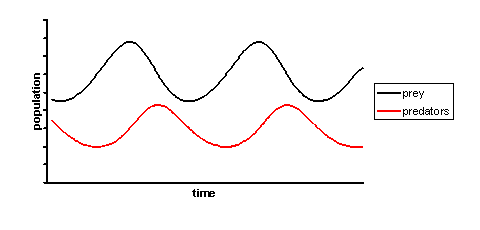
\includegraphics[width=0.8\textwidth]{G:/duke/courses/PHY566/hw7/evolution.png}
  \caption{}\label{Fig:evolution}
\end{figure}
Where, the peak of predator population is always $90^{\circ}$ ahead of that of prey population. \\
On the other hand, in mathematical prospect, the L-V equations have two solutions:
\begin{eqnarray*}
x &=& 0, y = 0 \\
or x &=& \frac{\gamma}{\delta}, y = \frac{\alpha}{\beta}
\end{eqnarray*}
Which is, either the two species will distinct, or they will reach a periodic stable situation. And, in the later situation, the evolution of the system doesn't depend on the size of the eco-system, or the initial numbers of two species. It only depends on the behavioral characteristics of the predator and the prey. \\
The result of this model matches with the evolution of our nature roughly. However, it can only simulate the situation when there's only one predator and one prey, it cannot simulate the situation when there are several predators in the eco-system, or several species are competing for one common resources. \\
When, several species are competing for a common resource, the competitive L-V equation can be adopted to modelize the situation:
\begin{eqnarray*}
\frac{dx}{dt} &=& \alpha_1 x (1- (\frac{x + \beta_{xy} y}{K_1})) \\
\frac{dy}{dt} &=& \alpha_2 y (1 - (\frac{y + \beta_{yx} x}{K_2}))
\end{eqnarray*}
The trophic interactions are included to the simulated system. \\
In addition, the generalized L-V equation can be used to model direct competition and trophic relationships between arbitrary number of species. But, in this study, we will just use L-V equation to produce a simple model between wolf and deer. \\

\section{Model description and implementation}
To simulate the interaction between the predator and pray we keep the essential features of the L-V equations:
\begin{enumerate}
	\item Procreation of deer and wolves when reproduction age is reached.
	\item Death of deer and wolves when starvation age is reached.
	\item Wolves feed on deer.
\end{enumerate}

We set up an animal class which generates instance of animals (deer and wolves), an animal takes record on its own age variables (reproducing age variable and starving age variable), its current and previous location. Animals can wander around an $N \times N$ grid world with periodic boundary condition (equivalent to the surface of a torus).

Initially, populations of deer and wolves with certain age structure is generated with each of their members occupied a randomly chosen but mutually exclusive position on the 2D gird. All the animal of the same species have the same age of sexual maturity and starvation.  A $N \times N$ occupation matrix tracks the position of all the animals, with vacant, deer, and wolves labeled by $0, 1$  and $2$ respectively. 

Within each step, the following operations are done serially: 
\begin{enumerate}
\item Step1: reproducing and starving age variable of each member of wolf and deer population are increased by $1$; then we check whether the starving age variable reaches the starvation age of this animal. Only if the animal is still alive shall we keep it in the animal list for the operations below.
\item Step2: loop over all wolf members and generate a list of its neighbours and take down its present location on the grid as previous location. If there is one or more deer around, then the wolf chooses one deer randomly and "eat" it by take over its spatial location and reset its own age back to zero. If there is no deer around but vacant position, the wolf move to one randomly chosen neighbouring position. The new position is then stored and compared with its previous location. If they are not equal and the wolves is mature, it deposits a new-born wolf at the vacant place left behind and reset its reproducing age variable to 0.
\item Step3: loop over all deer and check if its location is currently occupied by a wolf which means the deer is captured! Only those deer not captured will be kept in the animal list for the operations below.
\item Step4: loop over all deer left and move it to a randomly chosen vacant neighbouring position. If the new position is not equal to its previous location and the deer is mature, it deposits a new-born deer at the vacant position left behind and reset its own reproducing age to 0.
\item Step5: go back to Step1 and increase the system time by $1$
\end{enumerate}

We comment that as long as the steps above are done in serial manner there will be no conflict between the animals such as two wolves try to access to the same location or eat the same deer. Finally, there are a few remarks on the rule of choosing appropriate parameters in actual simulation: first the starvation age of deer is always chosen to be extremely large ($10^9$) so that deer will not die out of starvation; and second we restrict that the starvation age of wolves is always smaller than their reproduction age, or else the wolves population can maintain themselves simply by procreation and is totally independent on the presence of deer population, which is certainly unreal ( Although more realistic treatment do exist. For example, we can to assign each animal an "energy" such that zero energy sentence the animal to death and a certain portion of the energy must be transferred to its offspring during procreation.)

\section{Results and discussion}
\subsection{Parameter Search}
\indent
\indent The goal of this endeavour is to determine the parameters of our predator-prey system which provide a stable ecosystem.  In other words, we wish to find a 
system which satisfy the equilibrium condition of the Lotka-Volterra equations (i.e. when $\frac{dx}{dt} = \frac{dy}{dt} = 0$).  There are two possible solutions to 
this equilibirum condition: (1) when x=y=0 (the trivial solution), and (2) when $x=\frac{\gamma}{\delta}$ and $y=\frac{\alpha}{\beta}$ (non-trivial solution).  

There are many possible solutions to the non-trivial case.  Therefore, in order to determine a wide range of possible solutions, we attempt a full parameter search 
of our algorithm.  In this case, there are five parameters which must be explored simultaneously (5-D parameter space):
\begin{itemize}
  \item{Initial population of deer}
  \item{Initial population of wolves}
  \item{Reproduction age of deer}
  \item{Reproduction age of wolf}
  \item{Starvation "age" of wolf}
\end{itemize}
Since it is difficult to explore a 5-D space and represent it visually, we attempt to reduce the dimensionality of the parameter space by considering the 
relationship between the inital populations of the deer and the wolves, as opposed to their distinct values.  Therefore, we can reduce the dimension by taking 
the ratio between the deer and the wolf populations.  To display this visually, we take the reproduction age of the deer, the reproduction age of the wolf, and 
the starvation age of the wolf to be the cartesian axes in 3D, respectively.  The ratio of the populations is represented by the size of the point in our space.

To determine whether or not these parameters satisfy the equilibrium condition, we determine whether or not the populations are nonzero after a sufficiently long time. 
If a population is found to die out, then the data point is colored red.  On the other hand,if the populations do not die out after a certina amount of time, the 
ecosystem may be stable, so it is colored blue.

\subsection{Full Parameter Search}

\subsection{Restricted Parameter Search}
\indent
\indent Since the full parameter search did not yield any striking trends, we select fixed ratios of the initial deer and wolf populations.  The ratios chosen to provide 
a small sample were 10, 5, 1, 0.20, and 0.10. The results are shown below.

  \begin{figure}[H]
  \centering
        \begin{tabular}{@{}cc@{}}
                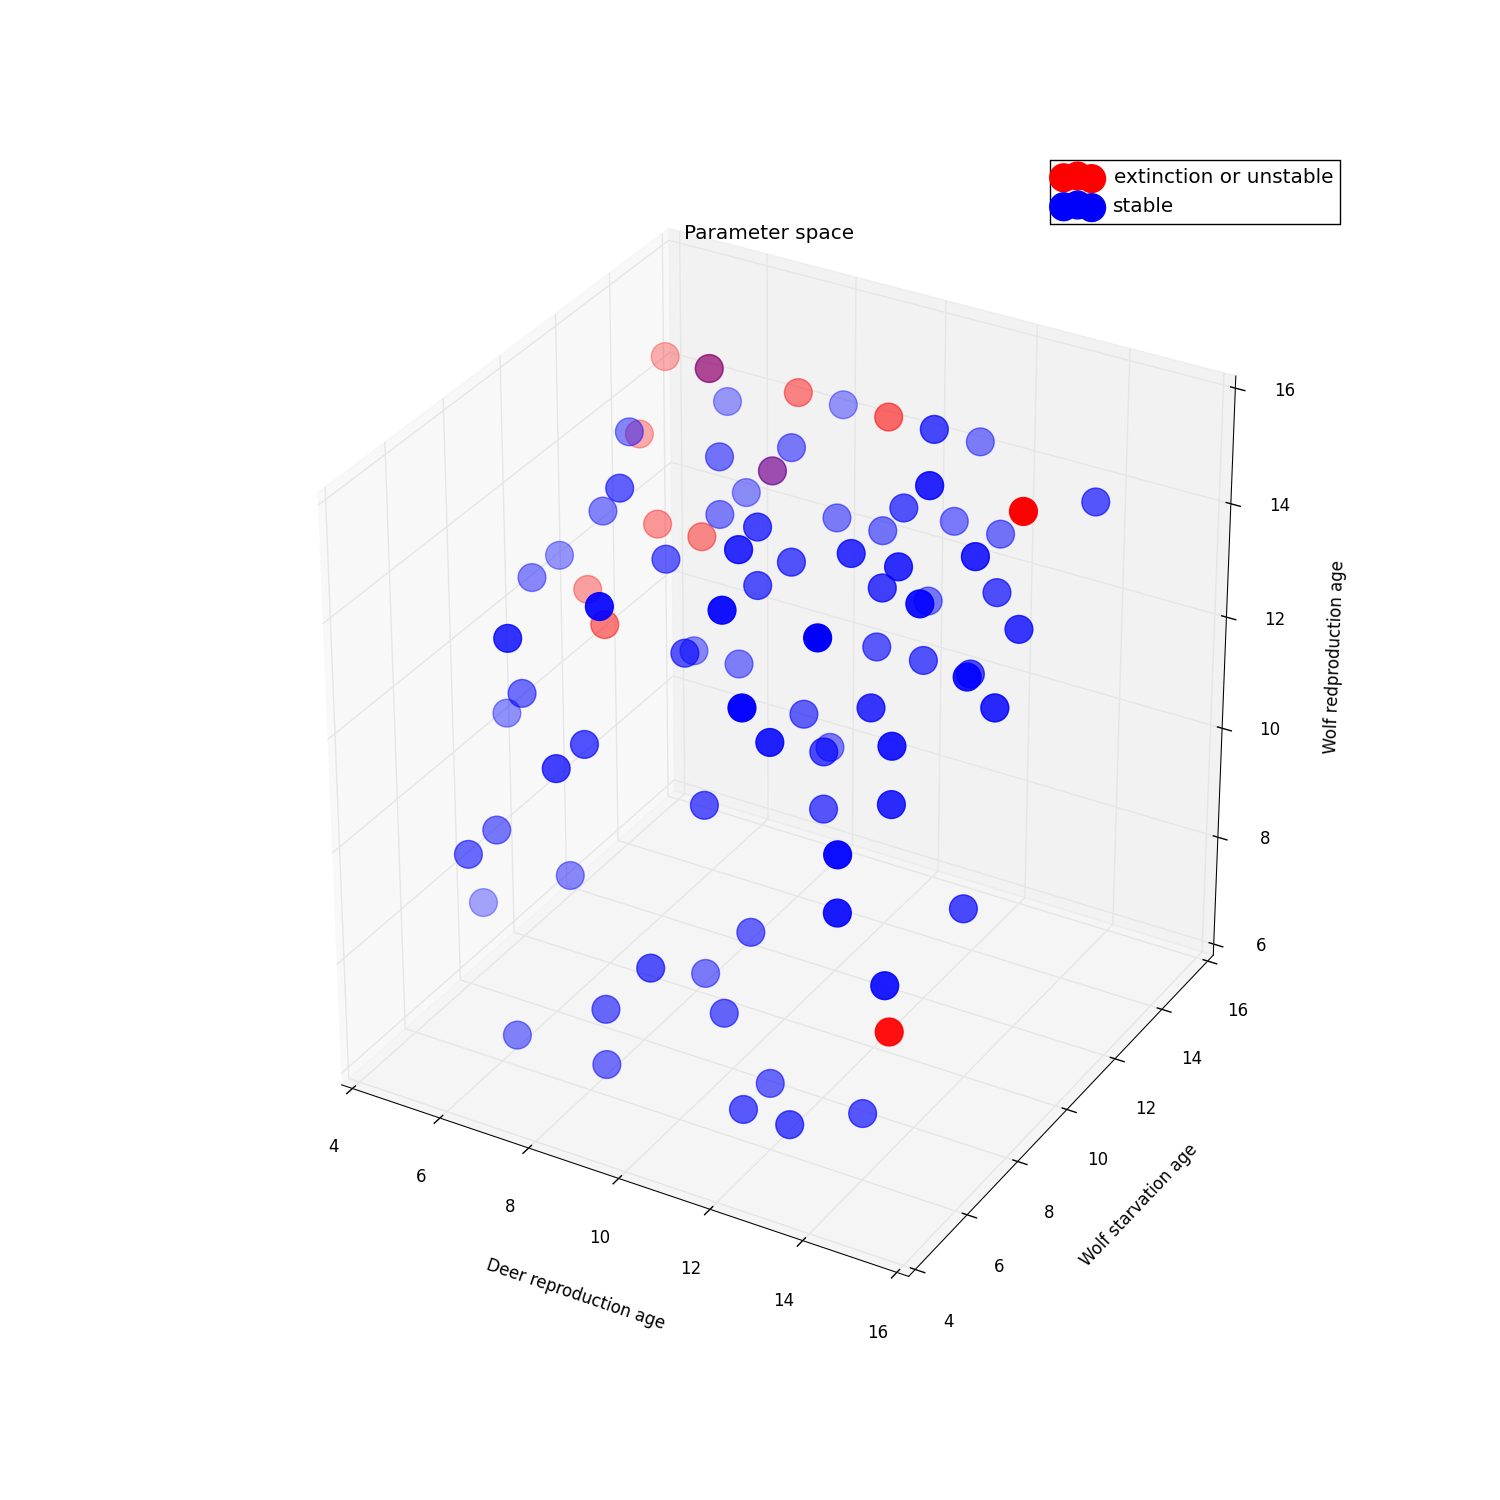
\includegraphics[width = 0.4\textwidth]{Restricted_Parameter_space_d2500_w250.png} &
                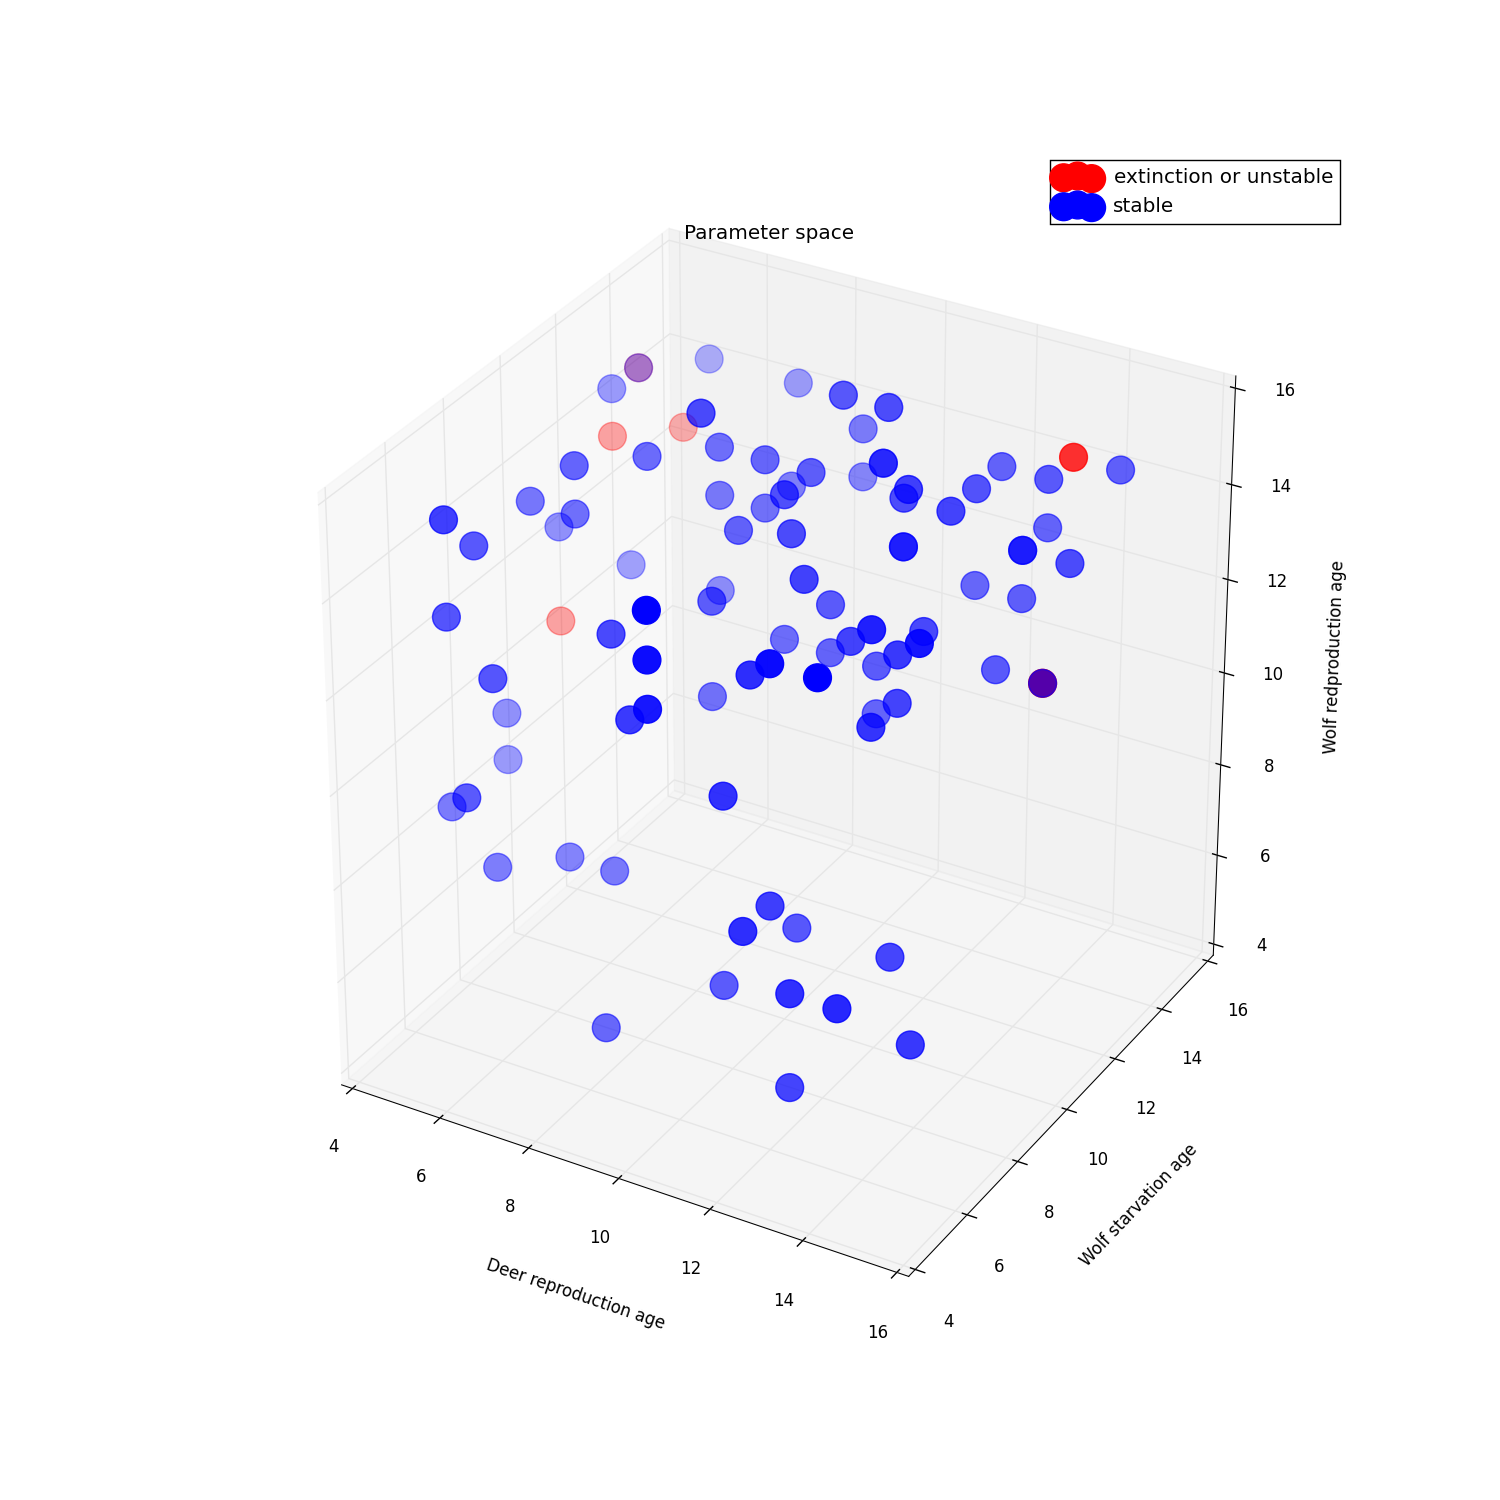
\includegraphics[width = 0.4\textwidth]{Restricted_Parameter_space_d3000_w500.png} \\
                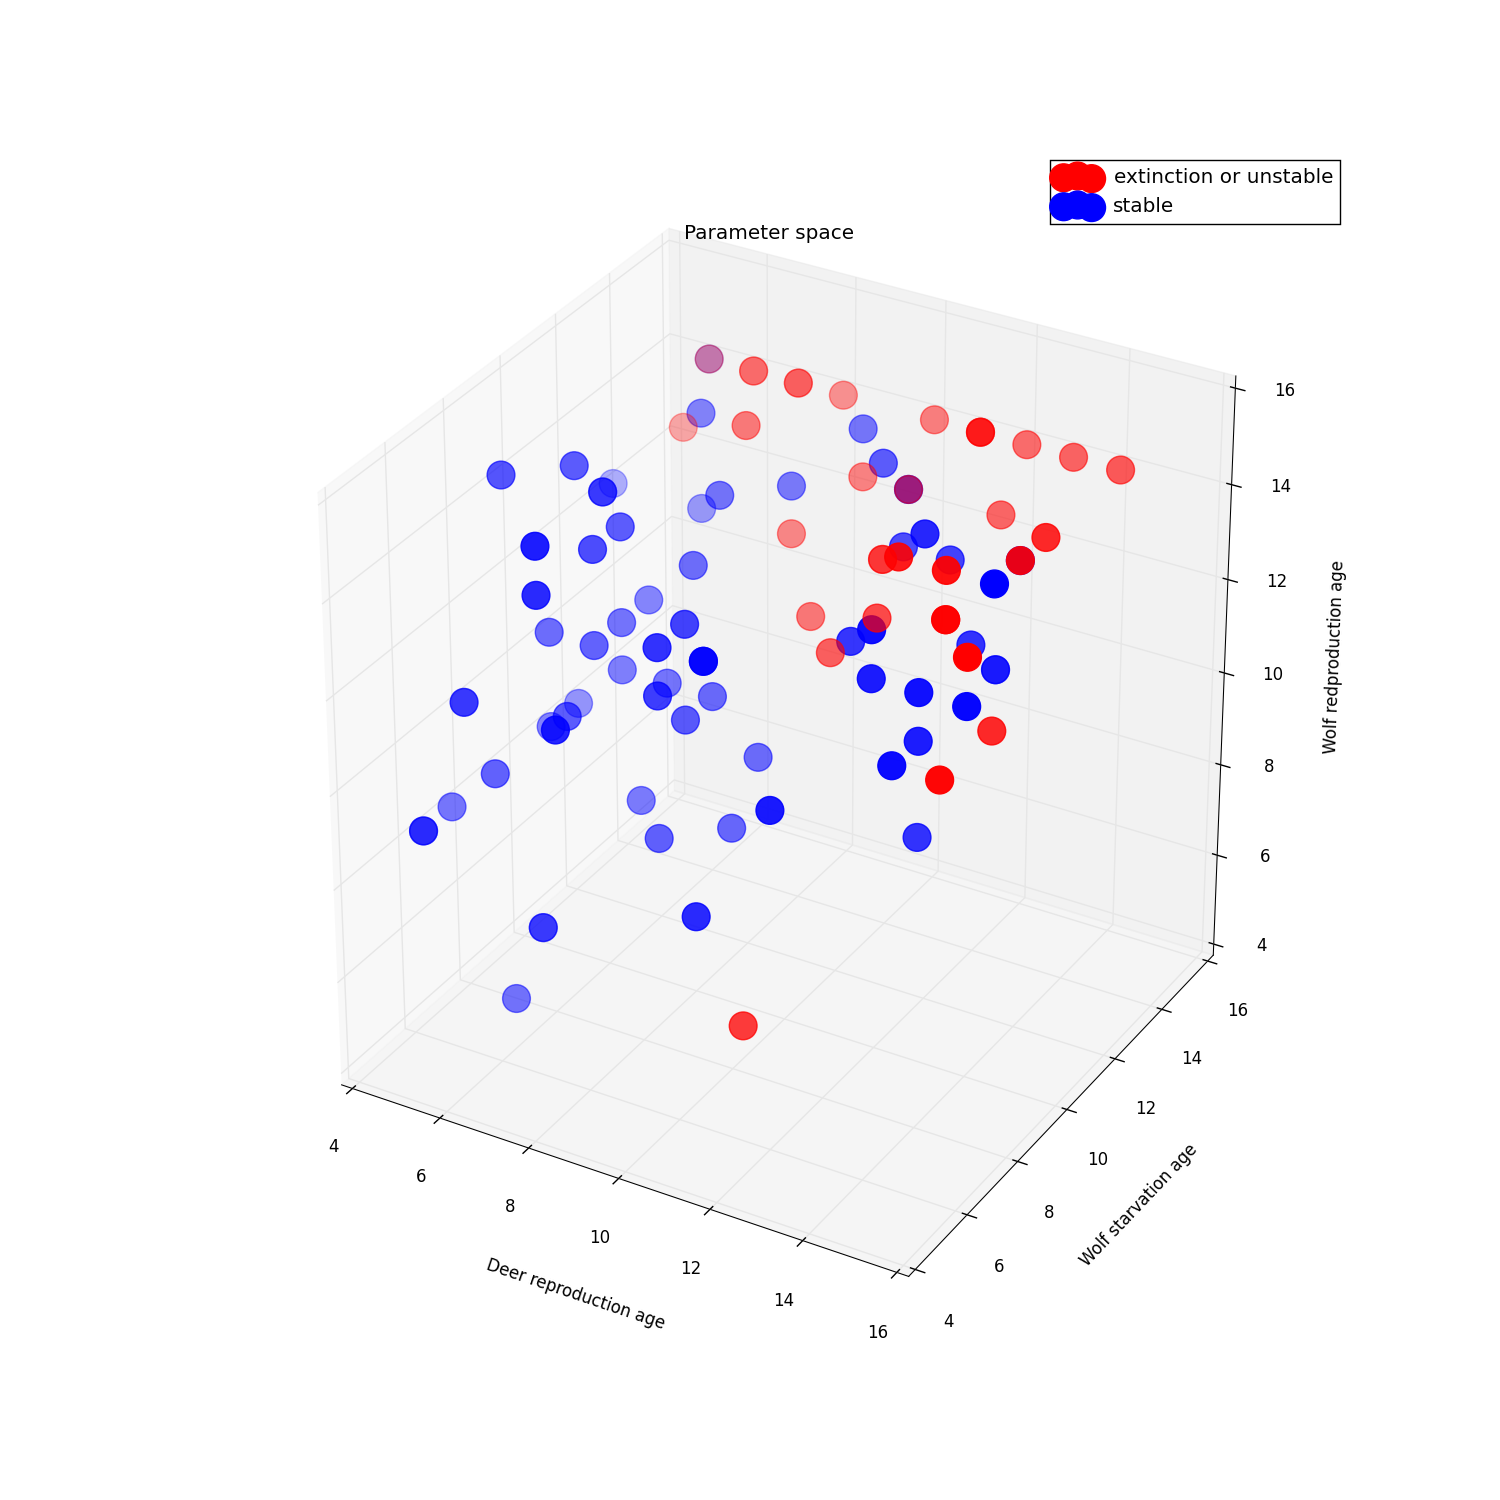
\includegraphics[width = 0.4\textwidth]{Restricted_Parameter_space_d2000_w2000.png} &
                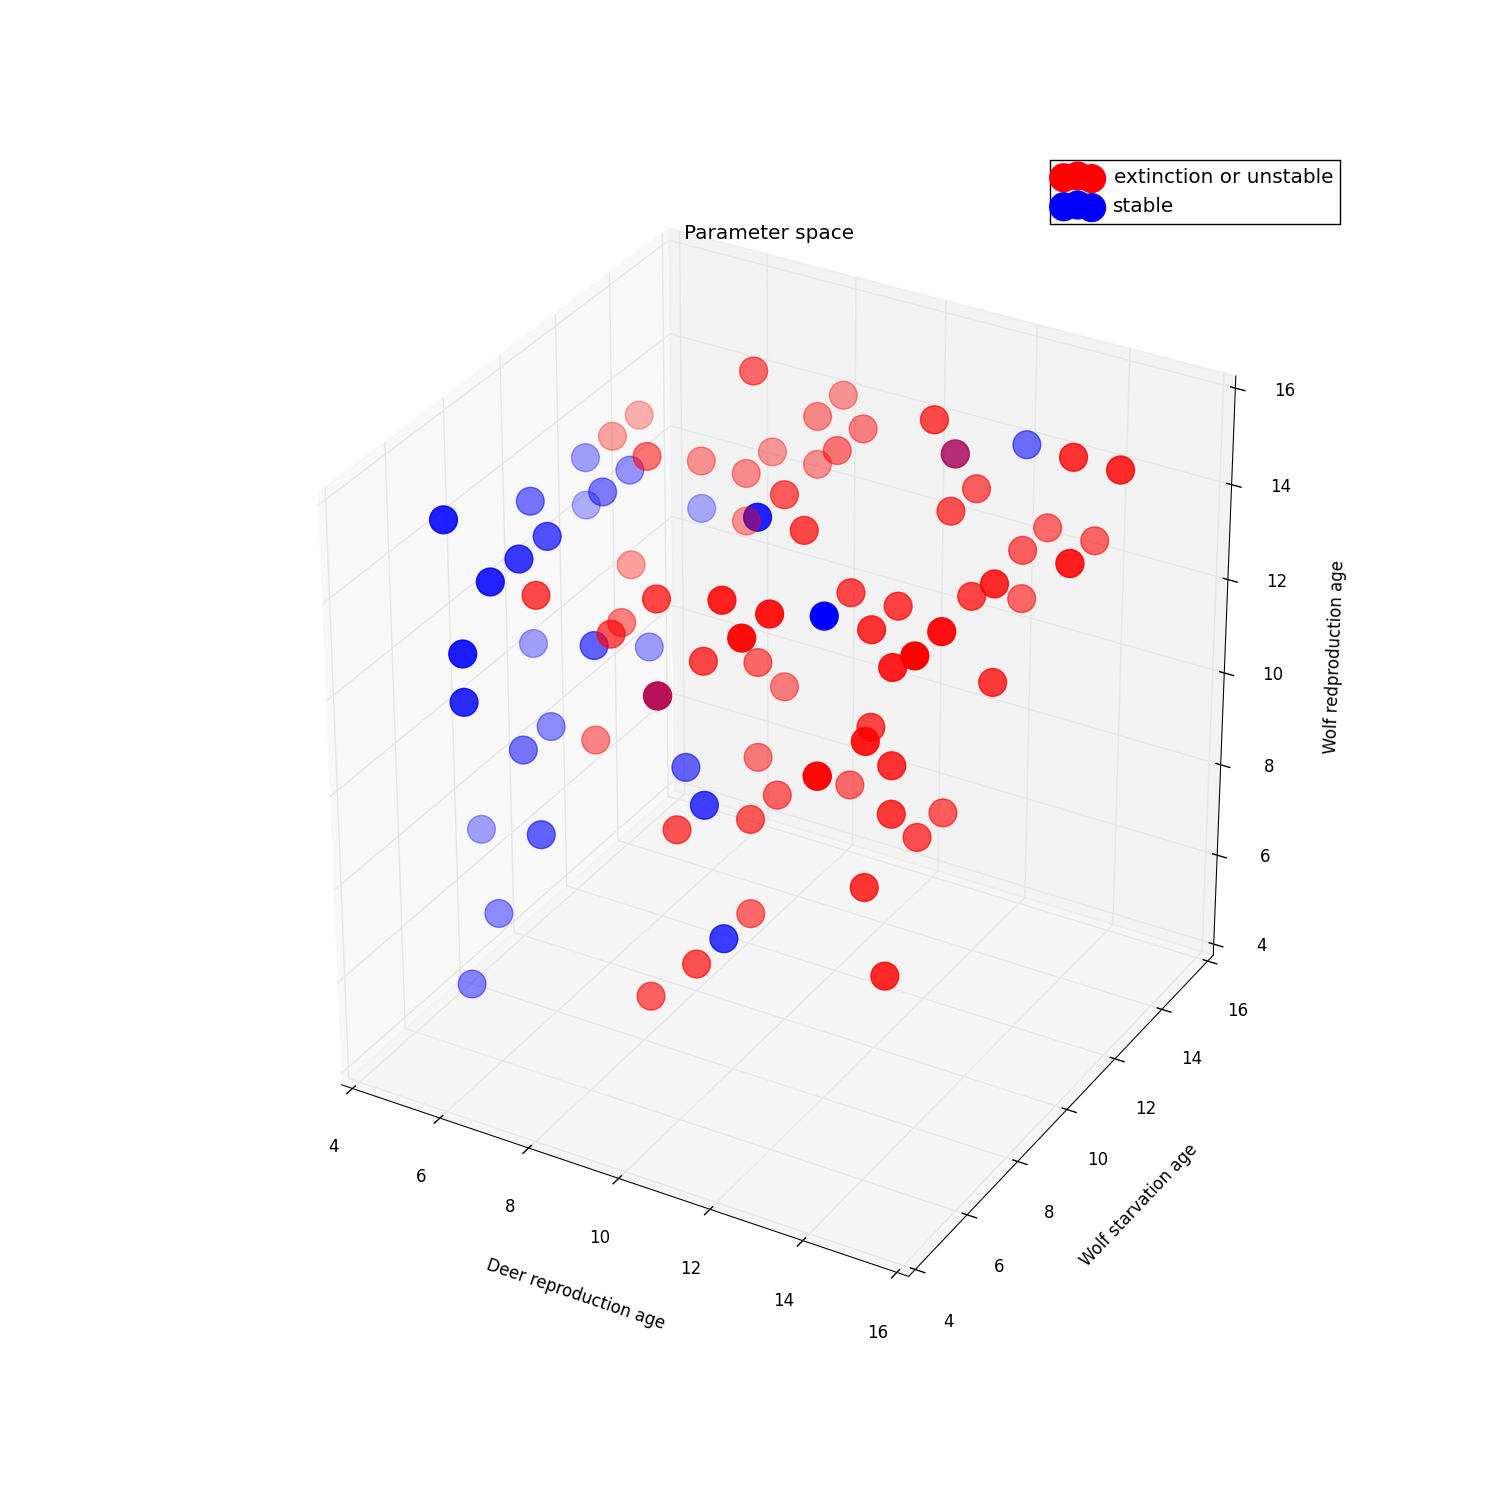
\includegraphics[width = 0.4\textwidth]{Restricted_Parameter_space_d500_w3000.png} \\
        \end{tabular}
        \label{RestrictParam}
  \end{figure}

\subsection{Stable System}
\indent
\indent Out of the possible stable configurations, one set of parameters was chosen to further exemplify a stable system.  The parameters used for the following 
stable system were (..................parameters.............).  Additionally, to show the dynamics of the system in "real-time" the python function \textit{
animation.FuncAnimation} was used to animate the ecosystem and display the 2D ecosystem after each time step.  (To view the animation, run the python code using 
method 1.)  However, snapshots of the system were taken at various intervals and are shown below.



Finally, from the Lotka-Volterra equations, we expect semi-sinusoidal behavior of our system at equilibrium.  When the predator population is at a maximum,
we expect the prey population to be a minimum and vise versa.  As a result, the populations were plotted as a function of time and are shown below.  



As expected, the populations exhibit a sinusoidal-type behavior with the population maxima and minima being opposite for each population.  Moreover, we notice
the behavior continues for the duration of the time shown.  Therefore, it is reasonable to assume an ecosystem with these parameters is expected to persist
over time, as long as there are no other outside influences.










 


 

\end{document}
